\section{Implementation}
\label{sec-implementation}
We will discuss Actors semantics in the context of a JVM-based Actor library called \af{}. \oaf{} was originally designed and developed at the Open Systems Laboratory by Mark Astley along with Thomas Clausen and James Waldby around 1998-2000 \cite{OAF}. The goal was to develop a modular Actor library for a new, upcoming object-oriented language called Java. \oaf{} has a simple, elegant model in which the control and mailbox are hidden away in the library while the programmer is concerned with an Actor's local state and behavior only \ref{actor_anatomy}. To leverage the actor semantics, the programmer is provided with a small set of library methods as part of the \oaf{} API. This includes:
\begin{description}
 \item[\code{send(actorAddress, message, args)}]
Sends an asynchronous message to the actor at specified address along with arguments. The argument message is a String which should match a method name in the target actor behavior, otherwise an exception is thrown at run-time.
 \item[\code{call(actorAddress, message, args)}]
Sends an asynchronous message and waits for a reply. The reply is also an asynchronous message which either contains the return value or simply an acknowledgement. 
 \item[\code{create(node, behavior, args)}]
Creates a new actor with the given behavior at the specified node. The argument node is optional. In case it is not specified, the actor is created locally. The arguments are passed to the constructor.
\item[\code{destroy(note)}]
An explicit termination of the current actor. This is provided as an alternative to an automatic actor garbage collection mechanism.
\item[\code{self()}]
Returns the address of the current actor.
\item[\code{migrate(node)}]
Requests the run-time to schedule the current actor for migration to a remote node. \oaf{} only supports weak mobility, hence the actor is migrated at message processing boundaries only.
\item[\code{cancelMigrate()}]
Cancels an earlier request for migration.
 \end{description}


Behind the scenes, \oaf{} maps each actor onto a JVM thread (1:1
architecture). Messages are dispatched to actors by using the Java
Reflection API. This can technically be termed as pattern-matching
since the message string is matched to a method name at run-time and
the method is selected based on the run-time type of arguments
\cite{multijava}. Though, it is certainly not as expressive as the
pattern-matching in Erlang \cite{erlang-book} and Scala
\cite{haller2007aut}. Any Java object can be part of a message in
\oaf{}; the only restriction being that the object implements
\code{java.lang.Serializable} interface. All message contents are sent
by making a deep copy by using Java's Serialization and
Deserialization mechanism.

\oaf{} also supports distributed execution of actor programs, location independence and weak mobility \cite{mobility}. In addition, \oaf{} logs system and library events to the local file system. 

%While this implementation faithfully preserves actor semantics like fairness (as fair as the underlying JVM and OS scheduler), encapsulation, location independence and mobility, it makes the execution overhead of actor programs prohibitively high, making \oaf{} infeasible to use. In order to gauge the performance of \oaf{}, we implement a small benchmark called Threadring \cite{lang-shootout} in which 503 concurrent entities pass a token around in a ring 10 million times. Threadring provides a crude estimate of actor creation overhead and stress tests the message-passing and context switch. When we ran this benchmark, it took about 780s \todo{verify on Amin's machine} to finish. In contrast, an Erlang implementation takes about 10s while a Java Thread implementation takes 150s \todo{verify on Amin's machine}.

This implementation faithfully preserves Actor semantics like fairness (as fair as the underlying JVM and OS scheduler), encapsulation, location independence and mobility. In order to gauge the performance of \oaf{}, we implement a small benchmark called Threadring \cite{lang-shootout} in which 503 concurrent entities pass a token around in a ring 10 million times. Threadring provides a crude estimate of actor creation overhead and stress tests the message-passing and context switch. 

For our experiments we use a Dell XPS laptop with Intel Core\texttrademark{} 2 Duo CPU @2.40GHz, 4GB RAM and 3MB L2 cache. The software platform is Sun's Java\texttrademark{} SE Runtime Environment 1.6.0 and Java HotSpot\texttrademark{} Server VM 10.0 running on Linux 2.6.26. We set the JVM heap size to 256MB for all experiments unless specified. Upon running this benchmark, we find it takes about 695s to finish. In contrast, an Erlang implementation takes about 8s while a Java Thread implementation takes 63s. See Figure \ref{tr_performance_orig_af} for a full comparison.
\begin{figure}%[htb]
%\begin{center}
\centerline
{
%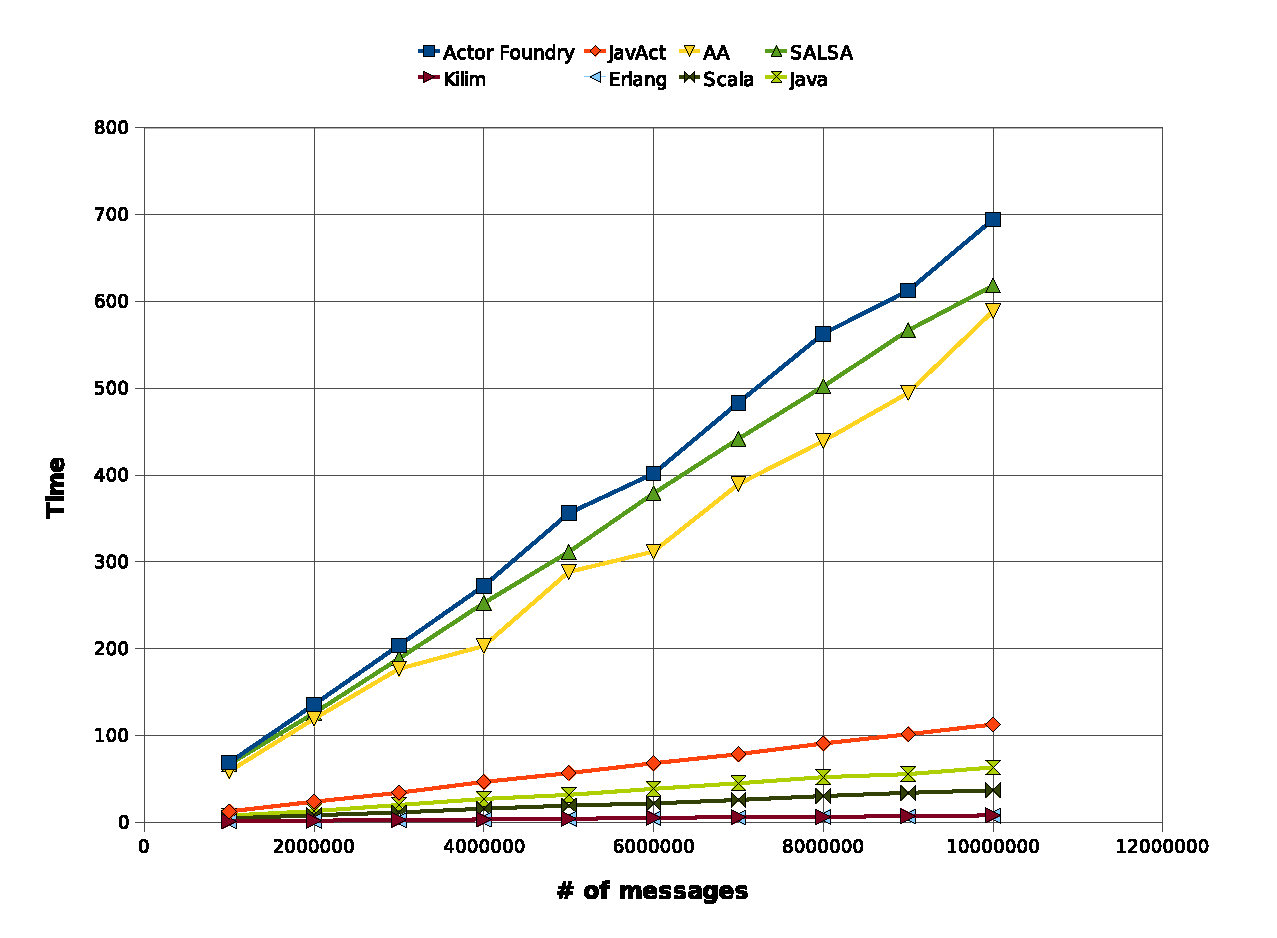
\includegraphics[bb=0 0 597 434, scale=0.55]{images/tr_performance_old_af.eps}
% tr_performance_old_af.eps: 0x0 pixel, 300dpi, 0.00x0.00 cm, bb=0 0 597 434
}
%\end{center}
\caption{Threadring Performance - \oaf{} compared with other concurrent languages and libraries}
\label{tr_performance_orig_af}
\end{figure}
This shows that a faithful but na\"ive implementation of Actor semantics can make the execution overhead of Actor programs extremely high, making \oaf{} feasible only for coarse-grained conccurent or distributed applications. We observe a similar execution overhead for SALSA and Actor Architecture. On the other hand, Kilim and Scala actors library perform an order of magnitude faster. JavaAct performs much better than \oaf{} but does not come close to either Kilim or Scala in terms of efficiency.

\subsection{Continuations based Actors}

Prior experience with ThAL language \cite{wkim-phd} suggests that continuations based actors would provide significant improvement in terms of creation as well as context switch overhead. We integrate Kilim's light-weight Task class and its bytecode post-processor (``weaver'') into \af{}. This transformation presents two challenges.

To begin with, the transform would not work when messages were dispatched using Java Reflection API. The reason being that the weaver is unable to transform Java library code and this prevented the continuations to be available in the actor code. To overcome this, we generate custom reflection for each actor behavior. It finds the matching method by comparing the message string to method's name and the type of message arguments to method's formal arguments' type. Once a match is found, the method is dispatched statically. As a pleasant side-effect, it is more efficient than Java Reflection. 

Secondly, the transform also require introducing a scheduler for \af{} which is aware of cooperative, continuations-based actors. The scheduler employs a fixed number of JVM threads called worker threads. All worker threads currently share a common scheduler queue. Each worker thread dequeues an actor from the queue and call its continuation. Actors are assumed to be cooperative; an actor continues to run until it yields waiting for a message. In order to increase locality and reduce actor context switches, an actor can process multiple messages while being scheduled. On the other hand, this can cause starvation in the system. Scheduling is message-driven only. An actor is put on the scheduler queue if and only if it has a pending message. 

With this implementation, the running time for Threadring comes down to about 267s.

\subsection{Message-passing semantics}
\label{messaging}

We profile the execution to identify further performance bottlenecks. Profiling makes it apparent that the deep copying of message contents is by far the biggest bottleneck. The faithful implementation of message-passing semantics means that message contents are deep-copied using Java's Serialization and Deserialization mechanism, even for immutable types. We disable deep-copying for some known immutable types. These included \code{java.lang.Integer}, \code{java.lang.String} and others. This further brings down the running time of Threadring to 30s. The reason behind this significant improvement is that actors in Threadring pass a token which is basically an integer representing the remaining number of passes.


We add two new methods to \af{} library: \code{sendByRef()} and \code{callByRef()} to overcome this inefficiency. These methods allow the programmer to explicitly declare transfer of ownership semantics for messages. This enables the run-time to implement such message efficiently on shared-memory systems by passing a reference.

\subsection{Na\"ive Implementation}
\subsubsection{Distribution and Location-Independent Addressing}
In \oaf{}, distributed execution is supported by means of a Transport layer. With its extensible architecture, either UDP or TCP based transport layer can be used. A node manager can communicate with another node manager by requesting its actor address through a lookup service called Yellow Page Service. The pre-requisite is that the service is running at the target node at the specified port. 

The client node can cache the manager's address locally. This address can now be used to send requests for creating actors remotely and migrating actors to the target node. This is where the power of location-independent addressing comes into play. Remote actor creation is a blocking operation that returns a location-transparent actor address. An actor on the client node can send send further messages to this actor on the remote node. It can also share this address with other actors and in turn they can send messages to this address without ever worrying about its physical location. 

In case a local actor migrates to a remote node, other actors that know this actor's address can continue to send messages to this actor. This location-independent addressing is enabled by using a protocol based on name tables, similar to the one discussed in \cite{sc95}.

\subsubsection{Mobility}
% Singularity: internal aliasing -> a complicated static analysis to ensure owernship transfer semantics

% TAlk about language based (Erlang run-time) implementation of these semantics. Static and Dynamic properties of Erlang process
\subsection{Optimizations}

